\chapter{Desenvolupament}
Un cop vist com funciona el protocol del Bluetooth Low Energy en aquest capítol s'analitzarà el dispositiu que l'implementa.
S'explicarà tant els components i parts que formen part del circuit imprès (\textit{Printed Circuit Board} o PCB d'ara endavant) com el programari que s'utilitza per desenvolupar projectes utilitzant-la.

\section{LaunchXL CC1352R1}
Per analitzar el protocol BLE i veure les seves característiques s'ha utilitzat el kit LaunchXL pel desenvolupament ràpid del microcontrolador CC1352R1.

\begin{figure}[h!]
	\begin{center}
		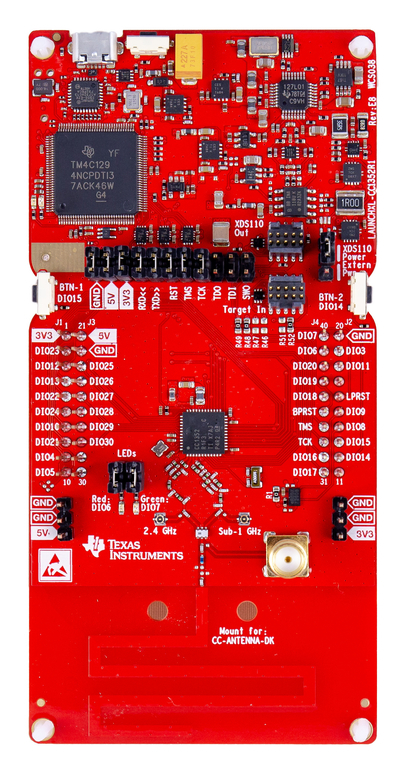
\includegraphics[width=0.5\textwidth]{./images/launchxl-cc1352r1.jpg}
		\caption{PCB amb la que es realitza el treball \cite{placa}}
		\label{PCB}
	\end{center}
\end{figure}

Aquesta PCB, que es pot veure a la figura \ref{PCB}, permet el desenvolupament d'aplicacions en BLE utilitzant el microcontrolador CC1352 de Texas Instruments a continuació es descriuen les seves característiques principals \cite{placa_datasheet}.

El dispositiu CC1352R és multiprotocol i multibanda orientat a 2.4 GHz o sub-1GHz que serveix per a Thread, Zigbee, Bluetooth 5 Low Energy, IEEE 802.15.4g i 6LoWPAN. Pel que fa a memòria té 352 KB flash programable, 256 KB de ROM per a protocols i llibreries, 8 KB de Cache SRAM i 80 KB de RAM protegida amb paritat.
Pel que fa als perifèrics el més important és el ADC de 12 bits i 8 canals amb freqüència de mostreig de 200 Kmostres/s (multiplexat). També té Rellotge de Temps Real (RTC en anglès), acceleradors d'operacions criptogràfiques i generador de números aleatoris.
La radio multibanda que té te un receptor amb sensibilitat de -121 dBm per a sub-1GHz i de -110 dBm a 50 Kbps o -105 dBm a 125 Kbps. El transmissor pot transmetre fins a 14 dBm sub-1GHz i 5dBm a 2.4 GHz.


\section{Software}
Per al desenvolupament de projectes per a la PCB s'ha utilitzat el entorn de desenvolupament Code Composer Studio 9. 
El CCS el distribuiex Texas Instruments i està basat en Eclipse \cite{eclipse}, que és de codi obert.
Aquest entorn de desenvolupament està orientat al desenvolupament per a processadors incrustats (\textit{embedded} en anglès) de les families fabricades per Texas Instruments.
El gran benefici d'aquest programa es que permet la depuració de programes basats en JTAG que es el cas d'aquesta PCB.

Tesxas Instruments té la plataforma SimpleLink que conté tant les llibreries necessaries per desenvolupar projectes com els recursos necessaris per a l'apranentatge de les tecnologies que es volen implementar.
Per poder realitzar projectes amb la PCB d'aquest treball és necessari utilitzar el SimpleLink CC13X2 versió 2.30.00.45\footnote{La versió utilitzada no és la més nova per a que sigui compatible amb la revisió C del xip que s'està utilitzant.}.

\section{Project 0}
El Project 0 és el projecte instal·lat amb que les PCBs vénen de fàbrica.
Aquest projecte exposa certs serveis a través de BLE i permet fer una comunicació simple entre la PCB i un dispositiu mòbil.
Aquesta comunicació es bidireccional, des del mòbil es poden controlar els LEDs que té la PCB.
I en el mòbil es pot veure si qualsevol dels dos botons esta pitjat.

Aquest projecte serveix per tenir un bon exemple de com està dissenyada l'arquitectura dels serveis amb les seves característiques amb una relativa simple funcionalitat. A continuació s'analitzaran diferents parts dels atributs.

\subsection{Serveis de Botons i LEDs}

En la taula \ref{tab:project_zero_uuid} es poden veure tots els valors que hi ha tal i com estan en la taula d'atributs del servidor GATT.
Per facilitar la visualització de les dades s'han tret els zeros finals dels UUIDs propis però cal recordar que en total tenen 16 parells de caràcters (128 bits en representació hexadecimal) i no només els 9 parells que surten a la taula.
\begin{table}[h!]
	\begin{center}
		\csvautotabular{data_files/projectzeroUUID.csv}
		\caption{Atributs del Project 0}
		\label{tab:project_zero_uuid}
	\end{center}
\end{table}
Els atributs en si no es poden identificar per tant és necessari tenir en compte la documentació del Project 0.
En la documentació hi ha inclosa una taula on es relaciona cada UUID amb el corresponent significat.

\begin{figure}[h!]
	\begin{center}
		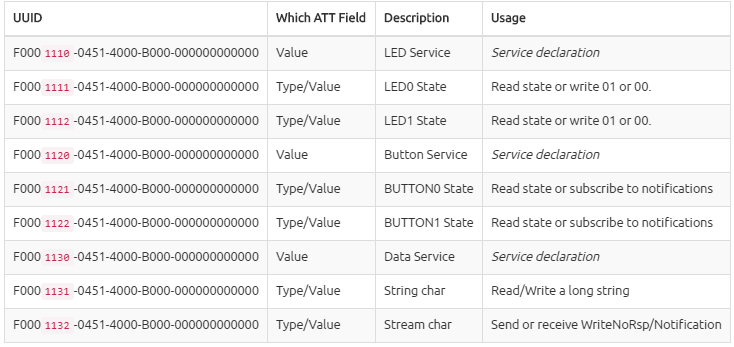
\includegraphics[width=\textwidth]{./images/Project_0_UUID.png}
		\caption{Definició dels UUIDs}
		\label{project0_table}
	\end{center}
\end{figure}

El primer que cal tenir clar és que en taula \ref{project0_table} els valors estan representats amb l'ordre en que es reben i en general els serveis estandarditzats (i també aquest servei propi) utilitza \textit{little-endian} per enviar la informació.
Això resulta en que els caràcters hexadecimals queden (per parelles, ja que, dos caràcters representen un byte) ordenats al revés.

Al analitzar els atributs es pot veure com aquells que tenen el UUID 0x2800 en el seu valor només tenen un UUID corresponent al les definicions de serveis de LEDs i de botons.
Seguidament, als atribut amb UUID 0x2803 hi ha les definicions de les característiques, en el seu valor hi ha múltiples parts.
El primer parell hexadecimal correspon a les propietats. Just després hi ha dos parells hexadecimals que identifiquen el \textit{Handle} del atribut on hi ha la característica.
I per últim la resta de caràcters corresponen al UUID que identifica la característica.

\subsection{Propietats}
\label{sec:properties}
Les propietats d'accés són un valor que identifica quines operacions i procediments es poden fer sobre la característica.
Es poden veure les propietats principals amb els corresponents valors en la taula \ref{properties}.
El camp té 8 bits per defecte i cada un d'ells identifica una operació o procediment.
Es poden combinar qualsevol quantitat d'aquests bits per habilitar múltiples opcions.

\begin{table}[h]
	\begin{center}
		\begin{tabular}{|c|c|l|}
			\hline
			Binary	&	Hex		&	Property	\\	\hline
			0000 0001	&	0x01	&	Broadcast\\	\hline
			0000 0010	&	0x02	&	Read	\\	\hline
			0000 0100	&	0x04	&	Write w/o Response	\\	\hline
			0000 1000	&	0x08	&	Write	\\	\hline
			0001 0000	&	0x10	&	Notification w/o ACK	\\	\hline
			0010 0000	&	0x20	&	Indication with ACK	\\	\hline
			0100 0000	&	0x40	&	Signed Writes	\\	\hline
			1000 0000	&	0x80	&	Aditional Properties	\\	\hline
		\end{tabular}		
	\end{center}
\caption{Valors de les propietats}
\label{properties}
\end{table}

Primer de tot cal destacar la implementació de comunicacions amb o sense reconeixement. D'aquesta manera si preferim reduir la quantitat de missatges per estalviar bateria enlloc d'assegurar-se que s'ha rebut la informació es dona l'opció.

Pel que fa les propietats en el Project 0 les característiques dels LEDs tenen el valor 0x0E que resulta en 0000 1110 per tant, es permet: llegir, escriure i escriure sense resposta.
En canvi les característiques del servei de botons té el valor 0x12 que suposa 0001 0010, per tant, es permet lectura i notificació sense reconeixement.

La notificació i indicació són funcions que ajuden a reduir el consum de recursos.
Quan volem saber en quin estat estan els botons de la PCB contínuament es podria anar llegint el estat de la característica constantment però això suposarien molts missatges i reduiria el temps que els dispositius es poden adormir i així ser més eficients.
Per evitar aquest cas es pot configurar la característica tal que sigui la mateixa PCB qui enviï el missatge automàticament quant el estat de la característica canviï.
D'aquesta manera el receptor només cal que escolti els missatges de la PCB per tal de saber en quin estat està el botó.

En cas de que es vulgui indicació amb reconeixements és possible configurar-ho d'aquesta manera a través del atribut Configuració de Característica del Client identificat amb el UUID 0x2902 i estandarditzat en la especificació de Bluetooth.
Si el valor és 0 no hi ha transmissions, si el valor és 1 s'envien notificacions (sense reconeixement) i si el valor és 2 s'envien indicacions (notificacions amb reconeixement). 

El bit d'extensió de propietats, en cas que sigui 1 indica que existeix un atribut: Descriptor Propietats Esteses de Característica.
Aquest atribut te el UUID 0x2900 i el que permet és afegir més propietats de les que poden existir amb el espai limitat de 8 bits que hi ha per defecte.
Aquest sistema permet afegir fins a 16 bits més per indicar propietats, actualment els dos primers es defineixen segons el estàndard i la resta estan reservats per a ús futur \cite{extended properties}.

Aquests 2 primers que estan definits són escriptura fiable i escriptura auxiliar.
L'escriptura fiable permet escriure valors amb un procediment diferent al habitual que permet assegurar-se que el valor que es vol modificar s'ha escrit i no hi han hagut errors.
Pel que fa a l'escriptura auxiliar, indica que es pot modificar un \textit{Characteristic User Description Descriptor} o CUDD.
En el CUDD hi ha descripcions definides per l'usuari com, per exemple, "Bombeta de la cuina".


\section{Client BLE}
Per poder interactuar amb un servidor de BLE és necessari tenir una implementació de client.
Com que els mòbils intel·ligents tots tenen BLE hi ha moltes aplicacions que permeten visualitzar els serveis amb les seves corresponents característiques.
També interactuar, escrivint o llegint aquells valors en que estigui permès.
Tot i així, no totes les aplicacions permeten rebre notificacions o utilitzar seguretat.
I les aplicacions no permeten interactuar directament amb el controlador (a través de HCI), per exemple, no poden canviar la potència de transmissió. 

Per poder tenir un control total del sistema l'equip de desenvolupament de programari que proporciona Texas Instruments conté l'aplicació BTool.
S'utilitza conjuntament amb el projecte Host Test del mateix equip per convertir la PCB en un client BLE.
El projecte Host Test permet controlar les diferents capes de la pila BLE del xip a través de la interfície sèrie.
Totes les possibles peticions, tant del servidor GAP com els missatges HCI.

\subsection{Btool}
L'aplicació BTool utilitza l'API del projecte Host Test per executar les crides a les diferents capes BLE.
Primer de tot, BTool necessita saber per quina interfície ha d'interactuar amb la PCB.
En l'administrador de dispositius de Windows es poden trobar els ports utilitzats per la PCB i els paràmetres de la connexió els indica Texas Instruments\cite{serial_params}.
Un cop s'inicia la comunicació entre BTool i la PCB es pot escanejar, iniciar connexió i descobrir la taula d'atributs del servidor.
En tot moment es poden veure tots els paquets que s'envien per la interfície amb la seva corresponent interpretació en la consola.
Com que en aquesta consola apareixen tots els esdeveniments de BLE 5, permet veure quan es reben notificacions.
Un cop s'ha establert la connexió es pot interactuar amb la taula d'atributs directament.


\section{Crear un Perfil propietari}

Per poder implementar una xarxa de sensors amb BLE serà necessari dissenyar un esquema propi en el servidor GATT.
Tal i com s'ha comentat anteriorment el servidor GATT està format per perfils que alhora agrupen serveis.
Aquests serveis son els que contenen les característiques amb les que s'interactuarà per intercanviar informació.
A continuació s'explicarà com es poden implementar perfils en l'entorn de Texas Instruments BLE Stack.

\subsection{Generar Fitxers}
Texas Instruments proporciona un Generador de Fitxers \cite{Service_Generator} que evita haver de començar de zero.
En aquesta eina s'han de definir el nom del servei, els noms de les característiques amb la seva longitud i les propietats i els corresponents UUIDs.
Aquesta eina està pensada per a ser utilitzada junt amb el Project Zero, per tant, aquest serà el projecte base per aquest treball.
Un cop s'han generat els fitxers cal copiar-los dins de Application/services en el projecte.

A parts dels fitxers generats (font i capçalera\footnote{Els fitxers de capçalera en C s'identifiquen per l'extensió .h i contenen les declaracions de funcions que es poden compartir entre múltiples fitxers font}) també cal que l'aplicació cridi a la funció que incialitza el servei registrant-los al GATT.
Aquesta és la funció [Perfil]\_AddService(..) que cal afegir dins la funció ProjectZero\_init() en la secció Inicialitació de Serveis.

Tot i que aquest generador de fitxers és molt útil a l'hora de tenir una estructura bàsica del projecte cal analitzar les parts importants per entendre com funciona per dins i quina relació té cada part amb BLE.

\subsection{Definir el Perfil Propi}
Per poder desenvolupar un perfil propi cal seguir els següents passos.

Cada característica necessita: un identificador per poderla classificar, el UUID que té assignat i la longitud de dades que tindrà.
Aquests valors es defineixen en el fitxer capçalera del perfil.

\begin{lstlisting}[language=C]
	#define TEMPERATURE_UUID 0x2345
	#define temperatureID 0
	#define temperatureLen 2
	
	#define humidityID 1
	#define humidityLen 2
	#define HUMIDITY_UUID 0x3456
	
	#define heartRate 2
	#define heartRateLen 2
	#define HEARTRATE_UUID 0x4567
	
	#define bloodOxygen 3
	#define bloodOxygenLen 2
	#define BLOODOXYGEN_UUID 0x5678
	
\end{lstlisting}

En aquest cas tots els UUIDs tenen 4 caràcters que suposen 16 bits. Però només es poden tenir UUIDs de 16 bits si estan reservats i aquest no és el cas.
Aquests 4 caràcters acabaran només sent part del UUID final que tindrà 128 bits un cop s'hagui afeigit farciment.
Això es fa utilitzant la funció TI\_BASE\_UUID\_128 que converteix els 16 bits a 128 amb el format F000XXXX-0451-4000-B000-000000000000 que és el que ve per defecte.

\begin{lstlisting}[language=C]
	CONST uint8_t environmentalServiceUUID[ATT_UUID_SIZE] =
	{TI_BASE_UUID_128(ENVIRONMENTALSERVICE_SERV_UUID)};
	
	CONST uint8_t temperatureUUID[ATT_UUID_SIZE]=
	{TI_BASE_UUID_128(TEMPERATURE_UUID)};
	
	CONST uint8_t humidityUUID[ATT_UUID_SIZE]=
	{TI_BASE_UUID_128(HUMIDITY_UUID)};
	
	CONST uint8_t heartrateUUID[ATT_UUID_SIZE]=
	{TI_BASE_UUID_128(HEARTRATE_UUID)};
	
	CONST uint8_t bloodoxygenUUID[ATT_UUID_SIZE]=
	{TI_BASE_UUID_128(BLOODOXYGEN_UUID)};
\end{lstlisting}

Posteriorment cal assignar l'espai necessari per poder emmagatzemar les dades de les característiques.

\begin{lstlisting}[language=C]
	static uint8_t temperatureVal[temperatureLen] = {0x00};
	static uint8_t tempProps = GATT_PROP_READ;
	
	static uint8_t humidityVal[humidityLen] = {0x00};
	static uint8_t humidityProps = GATT_PROP_READ;
	
	static uint8_t heartRateVal[heartRateLen] = {0x00};
	static uint8_t heartRateProps = GATT_PROP_READ;
	
	static uint8_t bloodOxygenVal[bloodOxygenLen] = {0x00};
	static uint8_t bloodOxygenProps = GATT_PROP_READ;
\end{lstlisting}

Tal i com es pot veure s'assigna tant espai com s'ha definit prèviament.
Els valors se'ls inicialitza a 0 i es defineix quines propietats tindran.

Una de les parts més importants de BLE i conseqüentment del servei és la taula d'atributs.
A continuació es pot veure com queda la taula definida en el codi\footnote{En aquest extracte de codi només s'inclouen la declaració del servei i les dues primeres característiques.}.

\begin{lstlisting}[language=C]
	static gattAttribute_t environmentalServiceAttrTbl[] =
	{
		{	{ ATT_BT_UUID_SIZE, primaryServiceUUID },
			GATT_PERMIT_READ,
			0,
			(uint8_t *)&environmentalServiceDecl	},
		{	{ ATT_BT_UUID_SIZE,  characterUUID},
			GATT_PERMIT_READ,
			0,
			&tempProps		},
		{	{ ATT_UUID_SIZE, temperatureUUID},
			GATT_PERMIT_READ,
			0,
			temperatureVal	},
		{	{ ATT_BT_UUID_SIZE,  characterUUID},
			GATT_PERMIT_READ,
			0,
			&humidityProps	},
		{	{ ATT_UUID_SIZE, humidityUUID},
			GATT_PERMIT_READ,
			0,
			humidityVal
		},
	};
\end{lstlisting}

La taula en codi està formada per un llistat d'atributs, la estructura d'aquests ve definida en el fitxer gatt.h i s'anomena gattAttribute\_t.
Cada objecte està format per quatre parts que són les següents:

- El UUID, al que cal afegir com a prefix la longitud que té.

- Les propietats que té l'atribut, que determinen quin tipus de permisos.

- El \textit{Handle} que cal deixar a 0 ja que s'assigna internament pel servidor.

- El valor en si del atribut que té una longitud màxima de 512 bytes
\newline

En cas de voler assignar més d'una propietat a la característica es pot fer utilitzant l'operador OR (en C correspon al símbol $\mid$).
Un exemple seria el següent: 
\begin{lstlisting}[language=C]
GATT_PERMIT_READ | GATT_PERMIT_WRITE
\end{lstlisting}
El fitxer gatt.h, que s'inclou dins del fitxer font, conté les definicions de tots els possibles permisos amb els seus valors en bits corresponents.

Per llegir o modificar els valors de les característiques és important fer-ho de forma segura i així evitar problemes com el desbordament de memòria intermèdia (\textit{Buffer Overflow} en anglès) que poden ocórrer si s'escriuen valors no vàlids.
Es per això que, en cada servei hi ha funcions de \textit{callback}.
Les funcions get i set s'utilitzen per llegir o modificar els valors que s'exposen a través de BLE.
Quant en algun punt del codi és necessari interactuar amb aquests valors es farà amb aquestes funcions.
Un exemple de la funció get és el següent:

\begin{lstlisting}[language=C]
bStatus_t EnvironmentalService_GetParameter(
	uint8_t param, uint8 len, void *value )
{
	bStatus_t ret = SUCCESS;
	switch ( param )
	{
		case temperatureID:
			memcpy(value, temperatureVal, len);
		case humidityID:
			memcpy(value, humidityVal, len);
		default:
			ret = INVALIDPARAMETER;
	}
	return ret;
}
\end{lstlisting}

En aquest exemple, es passa en els arguments: l'identificador de la característica (\textit{param}), la longitud d'aquesta (\textit{len}) i un punter on s'hi copiarà el valor (\textit{*value}).
La funció retorna un valor on indica si s'ha trobat o no la característica.

Per poder implementar notificacions cal que la característica tingui un \textit{Client Characteristic Configuration Descriptor} o CCCD.
El CCCD és un atribut més en la taula que cal posar just després del atribut on hi ha el valor de la característica i en codi quedaria de la següent manera\footnote{En aquest cas, l'exemple és del CCCD corresponent al boto 0 de la PCB que es troba al servei de botons del Project 0}.
\newline
\newline
\begin{lstlisting}[language=C]
{
	{ ATT_BT_UUID_SIZE, clientCharCfgUUID },
	GATT_PERMIT_READ | GATT_PERMIT_WRITE,
	0,
	(uint8_t *)&bs_BUTTON0Config
},
\end{lstlisting}

Com que el UUID correspon al de un CCCD cal que sigui 0x2902 que esta a la variable \textit{clientCharCfgUUID}.
La longitud del UUID és de dos bytes i s'indica amb la variable \textit{ATT\_BT\_UUID\_SIZE}.
La configuració per defecte es que s'enviaran notificacions a aquells dispositius que escriguin un 1 o Indicacions als que escriguin un 2.
Però per que el servidor sàpiga que ha de realitzar aquestes operacions cal executar la funció \textit{GATTServApp\_ProcessCharCfg} que ha d'estar en la funció set del servei.


%\subsection{Interactuar amb el hardware}

%Botons
%La placa que s'està utilitzant té dos botons que s'utilitzen com a entrades de senyals.
%En el fitxer principal project\_zero.c hi ha la funció ProjectZero\_handleButtonPress() que es crida quan es pressiona o es deixa de pressionar qualsevol dels botons.






